\documentclass[25pt, a0paper]{tikzposter}

%
%%%% pacotes adicionais
\usepackage{hyperref}
\usepackage{comment}
\usepackage{graphicx}
\usepackage{color, colortbl}
\usepackage{mathtools}
%
%%%% fontes
\renewcommand{\familydefault}{\sfdefault}
%
%%%% codificação e linguagem
\usepackage[utf8]{inputenc}
\usepackage[brazilian]{babel}



\definecolor{mygray}{HTML}{CCCCCC}
\definecolorstyle{myColorStyle} {
\colorlet{colorOne}{black}
\colorlet{colorTwo}{mygray}
\colorlet{colorThree}{gray}
}{
% Background Colors
\colorlet{backgroundcolor}{colorTwo!50}
\colorlet{framecolor}{colorTwo!50}
% Title Colors
\colorlet{titlefgcolor}{white}
\colorlet{titlebgcolor}{colorOne}
% Block Colors
\colorlet{blocktitlebgcolor}{colorThree!50}
\colorlet{blocktitlefgcolor}{black}
\colorlet{blockbodybgcolor}{colorTwo!50}
\colorlet{blockbodyfgcolor}{black}
% Innerblock Colors
\colorlet{innerblocktitlebgcolor}{white}
\colorlet{innerblocktitlefgcolor}{black}
\colorlet{innerblockbodybgcolor}{white}
\colorlet{innerblockbodyfgcolor}{black}
% Note colors
\colorlet{notefgcolor}{black}
\colorlet{notebgcolor}{white}
\colorlet{notefrcolor}{white}
}

\usebackgroundstyle{Default}
\usetitlestyle{Filled}
\usecolorstyle{myColorStyle}
\useblockstyle{Basic}
\usenotestyle{VerticalShading}

%Hide the latex tikzposter logo
\tikzposterlatexaffectionproofoff

\makeatletter
\centering
\renewcommand\TP@maketitle{%
    \begin{minipage}{0.1\linewidth}
       \centering
       \begin{tikzfigure}[]
            
\includegraphics[width=7.5cm,keepaspectratio]{./Imagens/cnpq} \\
            \vspace{1cm}
            
\includegraphics[width=7.5cm,keepaspectratio]{./Imagens/propesq}
            \vspace{0.1cm}
        \end{tikzfigure}
    \end{minipage}
    \begin{minipage}{0.8\linewidth}
        \centering
        \color{titlefgcolor}
        {\bfseries \huge \@title \par}
        \vspace*{1.5cm}
        {\LARGE \@author \par}
%       \vspace*{2em}
%        {\huge \@institute}
    \end{minipage}%
    \begin{minipage}{0.1\linewidth}
       \centering
       \begin{tikzfigure}[]
            
\includegraphics[width=7.5cm,keepaspectratio]{./Imagens/inf}
            \vspace{0.1cm}
        \end{tikzfigure}
    \end{minipage}
}
\makeatother


\title{\parbox{\linewidth}{\centering Análise de Conflitos e Dependências em Modelos Computacionais baseados em Transformações de Grafos \\ \vspace{15pt} \large Trabalho realizado com o apoio da Pró-Reitoria de Pesquisa - UFRGS e Conselho Nacional de Desenvolvimento Científico e Tecnológico (CNPq)}}%%

\author{Leonardo Marques Rodrigues, Orientação: Prof. Dra. Leila Ribeiro}


\begin{document}

\maketitle%
\begin{columns}%
    \column{0.5}
        \block{Introdução}{
            \LARGE        
            \emph{Gramáticas de grafos}\cite{ehrig2006} são modelos visuais com os quais pode-se descrever sistemas, onde os estados são modelados através de grafos e o comportamento como regras de reescrita de grafos, chamadas de \emph{regras de transformação}. A utilização desses modelos para a aplicação de métodos de verificação formal permite aliar uma apresentação visual e intuitiva com uma semântica de execução precisa. Dentre as análises que podem ser feitas sobre gramáticas de grafos encontra-se a análise de par crítico. Essa é uma análise estática que visa determinar todas as possíveis interações entre pares de regras, identificando situações como conflitos ou dependências. O uso de gramática de grafos pode ser empregado no estudo de diversas áreas, tais como modelagem de sistemas concorrentes e distribuídos, design de banco de dados, construção de compiladores e muitos outros.
        }

        \block{Desenvolvimento}{
            \LARGE 
            O projeto \emph{Verites}\cite{verites}, está desenvolvendo uma nova ferramenta para edição, execução e verificação de modelos utilizando gramáticas de grafos, denominada \emph{Verigraph}\cite{verigraph}. Essa ferramenta visa integrar todas as funcionalidades necessárias para análises  em gramática de grafos, o que é uma carência das ferramentas disponíveis (especializadas em somente um tipo de análise). Atualmente a ferramenta \emph{Verigraph} já possui funcionalidades importantes implementadas, como análise de conflitos e dependências entre regras e cálculo de regra concorrente a partir de uma derivação. Estão sendo implementadas atualmente funcionalidades adicionais como Verificação de Modelos (utilizando a lógica \emph{CTL}) e suporte a gramáticas de grafos de 2º ordem. \\
 
            Durante o desenvolvimento deste trabalho minhas contribuições para a ferramenta se concentraram na implementação da verificação de \emph{matches} (aplicabilidade das regras), na análise e comparação de desempenho com ferramentas já existentes e também no auxilio à implementação dos módulos de Análise de Conflitos e Dependências.
        }

        \block{Gramática de Grafos}{
            \LARGE
            Uma \emph{Gramática de Grafos Tipados}\cite{ehrig2006} é uma tupla $\mathcal G = (T,G_0,P,\pi)$, onde $T$ é um grafo (Grafo Tipo), $G_0$ é um grafo tipado em T (Grafo Inicial), $P$ é um conjunto de nomes de regras de transformação e $\pi$ é uma função que associa cada nome pertencente a $P$ a uma regra de transformação. \\

            Uma regra de transformação\cite{ehrig2006} é uma tupla $\mathcal P = (N,L\xleftarrow{l} K \xrightarrow{r} R)$, sendo $l : K \to L$ e $r: K \to R$ homomorfismos de grafos injetores e $N = \{ n_i : L \to X_i \}$ uma coleção de morfismos com origem em $L$. O grafo tipado $L$ representa o padrão de aplicação de uma transformação, $R$ representa o padrão resultante de uma transformação e $N$ representa um conjunto restrições na aplicação da transformação.

        }

    \column{0.5}

        \block{Estudo de Caso}{
            \LARGE
            Para ilustrar o funcionamento de uma modelagem com Gramática de Grafos, abaixo é listado um exemplo modelando a transformação de uma árvore binária qualquer em uma lista. \\

            \begin{center}
                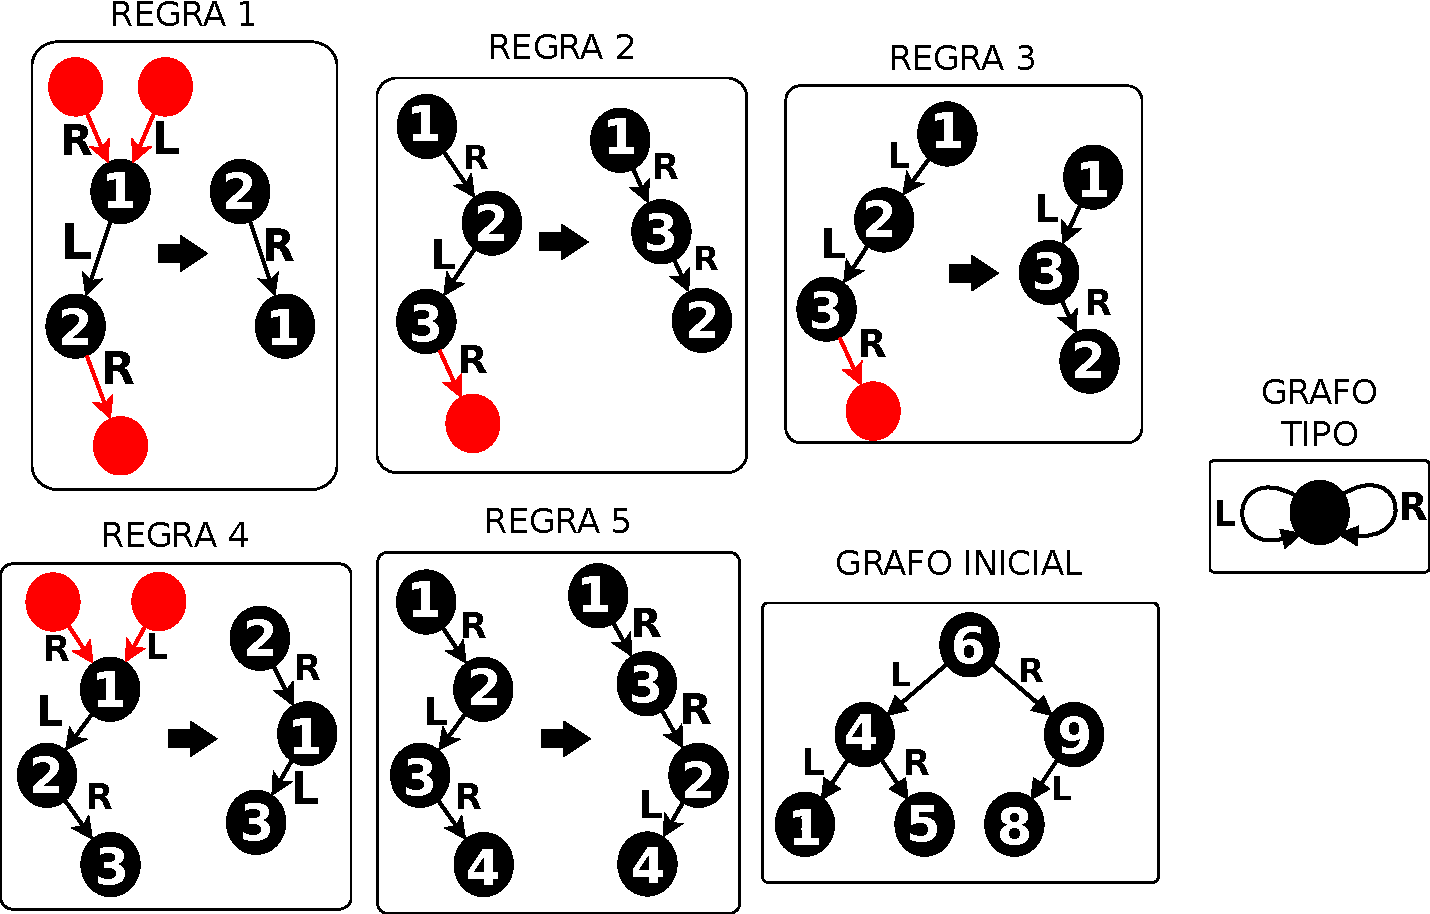
\includegraphics[height=17.5cm,keepaspectratio]{./Gramatica/TreeToList.pdf} \\
                {\large *Símbolos vermelhos representam restrições de aplicações}
            \end{center}
            \vskip 1cm

            Para simular o comportamento do sistema, as regras são aplicadas sucessivamente sobre o grafo inicial, até que nenhuma das regras seja aplicável. Abaixo está um exemplo da aplicação da Regra 2 no Grafo Inicial: \\

            \begin{center}
                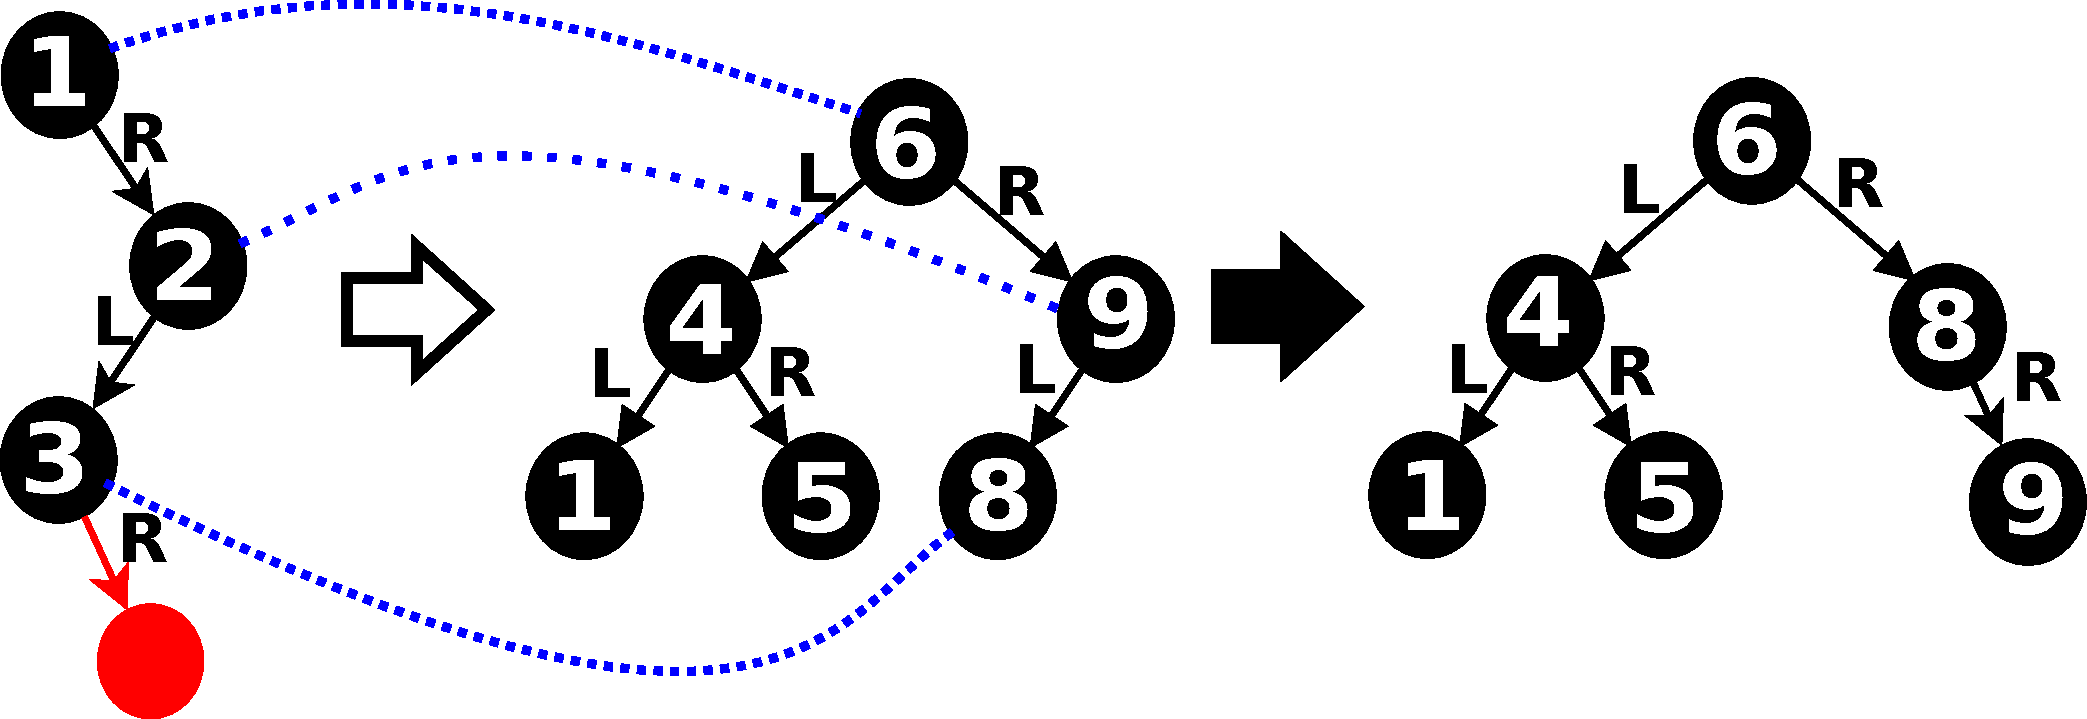
\includegraphics[height=7.5cm,keepaspectratio]{./Gramatica/Application_Rule1.pdf}
            \end{center}

            A execução da gramática a seguir, aplicando-se a sequência de regras formada pelas regras 2, 4, 1 e 2 ao grafo inicial resulta no seguinte grafo final:
            \begin{center}
                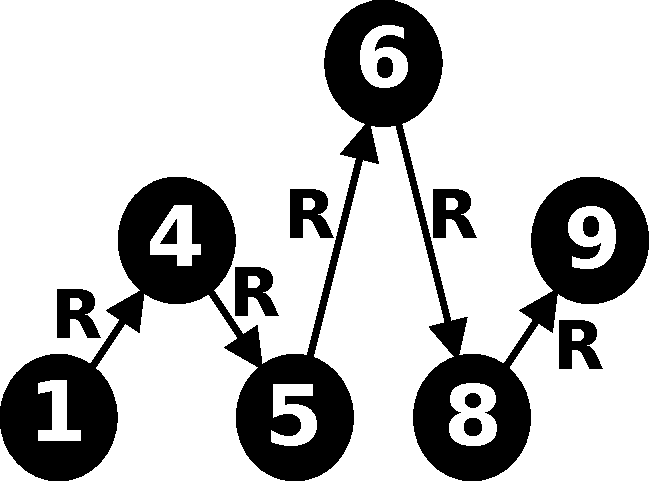
\includegraphics[height=6.5cm,keepaspectratio]{./Gramatica/Final.pdf}
            \end{center}

            \LARGE
            Dentre as possíveis análises que podem ser feitas sobre gramáticas de grafos encontra-se a análise de par crítico, que visa determinar as interações entre pares de regras, identificando situações de conflitos ou de dependências. Essa análise é útil pois permite uma visão geral sobre as interações entre todas as regras, apontando principalmente onde a execução concorrente das regras é inviável. Abaixo, estão os resultados das Análises de Conflitos e Dependências realizadas na gramática apresentada:

            \begin{center}
                \begin{minipage}{0.45\linewidth}
                    \small \centering
                    \begin{tikzfigure}[]

                    \newcolumntype{g}{>{\columncolor{colorThree}}c}
                    \newcommand{\green}{\cellcolor{green!25}}
                    \newcommand{\red}{\cellcolor{red!25}}

                    \begin{tabular}{|g|c|c|c|c|c|}
                        \hline
                        \rowcolor{colorThree}
                        $\backslash$ & ~R1~ & ~R2~  & ~R3~  & ~R4~  & ~R5~  \\ \hline
                        ~R1~         & \red 3 & \red  1 & \red 2  & \red  1 & \green  0 \\ \hline
                        ~R2~         & \red 5 & \red 10 & \red 9  & \red  7 & \red  5 \\ \hline
                        ~R3~         & \red 5 & \red  7 & \red 12 & \red  7 & \red  4 \\ \hline
                        ~R4~         & \red 4 & \red  5 & \red 5  & \red 10 & \red  5 \\ \hline
                        ~R5~         & \red 5 & \red 13 & \red 12 & \red 17 & \red 42 \\ \hline
                    \end{tabular}
                    \end{tikzfigure}
                    {Resultado da Análise de Conflitos}%
                \end{minipage}
                \begin{minipage}{0.45\linewidth}
                    \small \centering
                    \begin{tikzfigure}[]

                    \newcolumntype{g}{>{\columncolor{colorThree}}c}
                    \newcommand{\green}{\cellcolor{green!25}}
                    \newcommand{\blue}{\cellcolor{blue!25}}

                    \begin{tabular}{|g|c|c|c|c|c|}
                        \hline
                        \rowcolor{colorThree}
                        $\backslash$ & ~R1~    & ~R2~     & ~R3~     & ~R4~     & ~R5~     \\ \hline
                        ~R1~         & \blue 1 & \blue  1 & \green 0 & \blue  2 & \blue  2 \\ \hline
                        ~R2~         & \blue 3 & \blue  5 & \blue  2 & \blue  7 & \blue 12 \\ \hline
                        ~R3~         & \blue 2 & \blue  3 & \blue  3 & \blue  7 & \blue  8 \\ \hline
                        ~R4~         & \blue 4 & \blue  5 & \blue  4 & \blue  7 & \blue  8 \\ \hline
                        ~R5~         & \blue 5 & \blue 18 & \blue 13 & \blue 18 & \blue 37 \\ \hline
                    \end{tabular}
                    \end{tikzfigure}
                    {Resultado da Análise de Dependências}%
                \end{minipage}

            \end{center}
        }
        
        \block{Referências}{
            \large
            \begingroup
                \renewcommand{\section}[2]{}
                \bibliographystyle{plain}
                \bibliography{poster.bib}
            \endgroup
        }%
        
\end{columns}
\end{document}
